\documentclass[11pt,a4paper]{article}

\usepackage[utf8]{inputenc}
\usepackage[T1]{fontenc}
\usepackage[spanish]{babel}
\usepackage{graphicx}
\usepackage{booktabs}
\usepackage{float}
\usepackage{caption}
\usepackage[margin=2.2cm]{geometry}
\usepackage{subcaption}

\captionsetup{font=small,labelfont=bf}
\setlength{\parskip}{4pt}
\setlength{\parindent}{0pt}

\title{\vspace{-1.5cm}\textbf{Trabajo Pr\'actico 3 --- Visi\'on Computacional con CNNs}\\
\large Clasificaci\'on de im\'agenes satelitales EuroSAT (PyTorch)}
\author{Juan Ignacio Elosegui \quad Juan Gonz\'alez Merlhe \\
\small Tecnolog\'ia Digital VI --- Inteligencia Artificial}
\date{\vspace{-0.3cm}\small Junio 2026}

\begin{document}
\maketitle
\vspace{-0.6cm}

\section{CNN propia entrenada desde cero}

\textbf{Arquitectura.} Dise\~namos una CNN de 4 bloques convolucionales, cada uno con el patr\'on
\texttt{Conv($3\times3$) $\to$ BatchNorm $\to$ ReLU $\to$ MaxPool}, que duplica los canales
($3\to32\to64\to128\to256$) mientras reduce la resoluci\'on espacial de $64\times64$ a $4\times4$.
En lugar de aplanar el mapa de features usamos \emph{Global Average Pooling}, seguido de una cabeza
densa ($256\to128\to10$) con \texttt{Dropout}. El modelo tiene apenas \textbf{423.562 par\'ametros},
muy compacto. BatchNorm y Dropout act\'uan como regularizadores y estabilizan el entrenamiento.

\textbf{Pipeline de datos y \emph{data augmentation}.} Cargamos los datos con \texttt{Dataset}/\texttt{DataLoader}.
Sobre el conjunto de entrenamiento aplicamos aumentaciones acordes a la naturaleza satelital de las
im\'agenes, donde no existe una orientaci\'on privilegiada: \emph{flips} horizontal y vertical,
rotaciones de hasta $90^\circ$ y un \texttt{ColorJitter} suave de brillo/contraste/saturaci\'on.
Estas transformaciones explotan las invarianzas geom\'etricas del dominio y reducen el sobreajuste.
Validaci\'on y test usan \'unicamente normalizaci\'on (evaluaci\'on determin\'istica).

\textbf{Entrenamiento y monitoreo.} Entrenamos 30 \'epocas con Adam (\texttt{lr}$=10^{-3}$,
\texttt{weight\_decay}$=10^{-4}$) y \texttt{ReduceLROnPlateau}, optimizando \emph{cross-entropy}.
La Figura~\ref{fig:train-custom} muestra la evoluci\'on de \emph{loss} y \emph{accuracy} en train y
validaci\'on: la curva de validaci\'on es ruidosa pero con tendencia creciente hasta estabilizarse
en torno al $0{,}94$ de \emph{accuracy}.

\begin{figure}[H]
    \centering
    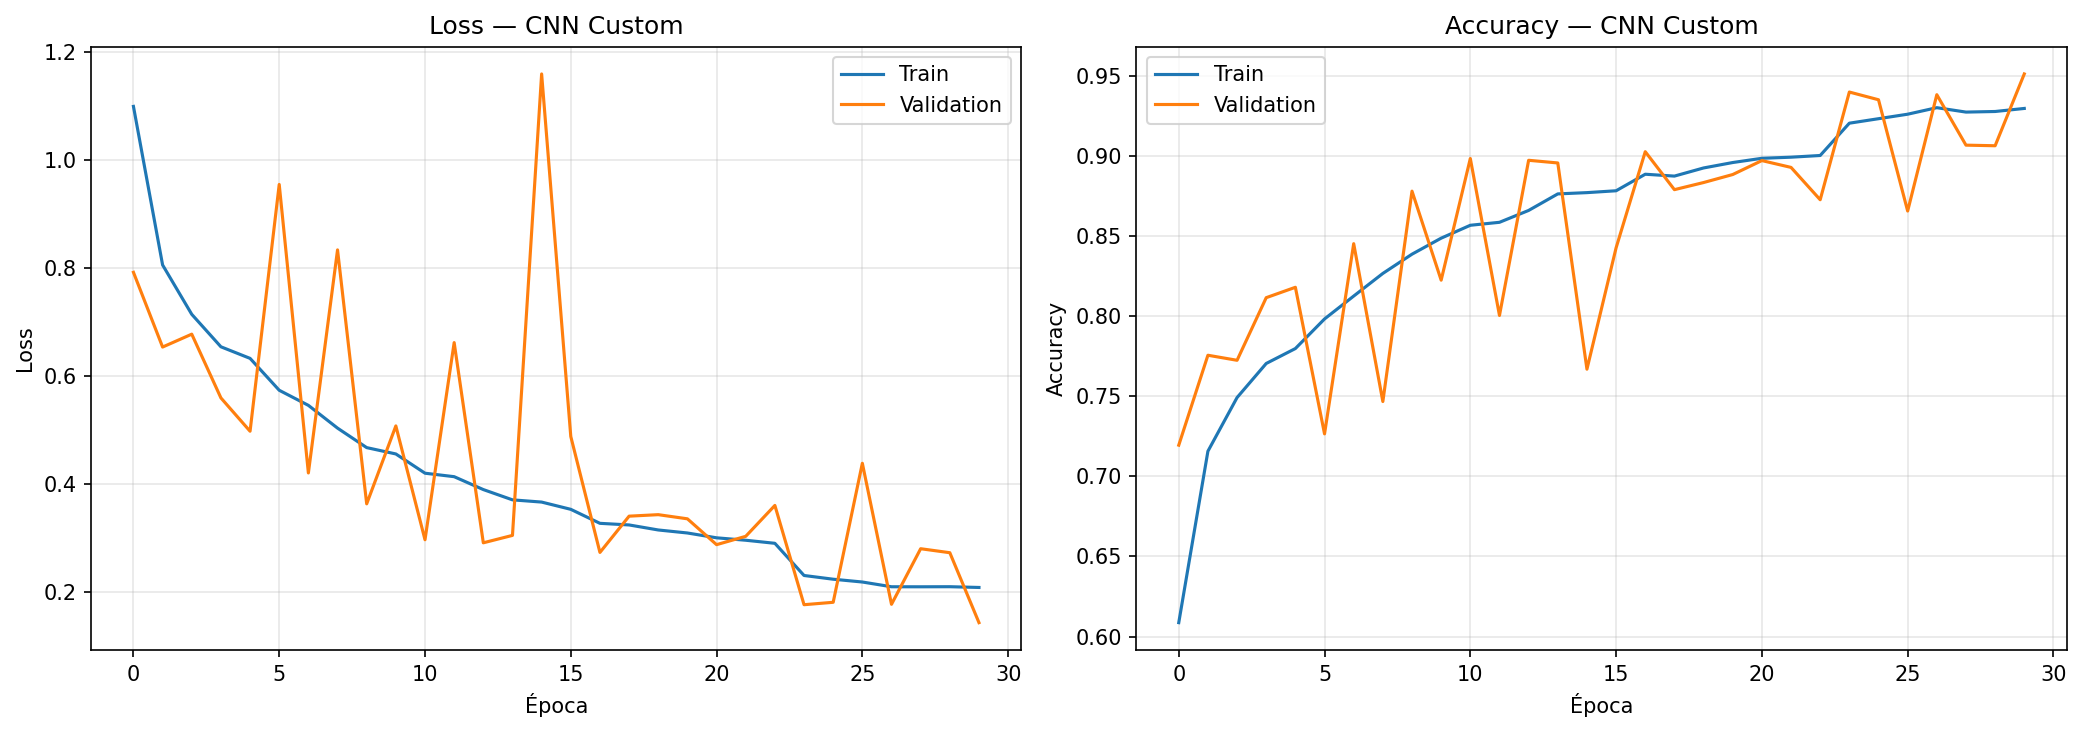
\includegraphics[width=0.80\linewidth]{training_cnn_custom.png}
    \caption{Evoluci\'on de \emph{loss} y \emph{accuracy} (train vs.\ validaci\'on) de la CNN propia.}
    \label{fig:train-custom}
\end{figure}

\textbf{Flujo de gradientes.} Para descartar \emph{vanishing}/\emph{exploding gradients} registramos la
norma del gradiente por capa durante las primeras \'epocas (Figura~\ref{fig:grads}). Las normas se
mantienen acotadas en un rango sano ($\sim10^{-1}$ a $\sim10^{1}$), sin colapsar a cero ni dispararse:
BatchNorm cumple su rol y el flujo de gradientes es estable en toda la red.

\begin{figure}[H]
    \centering
    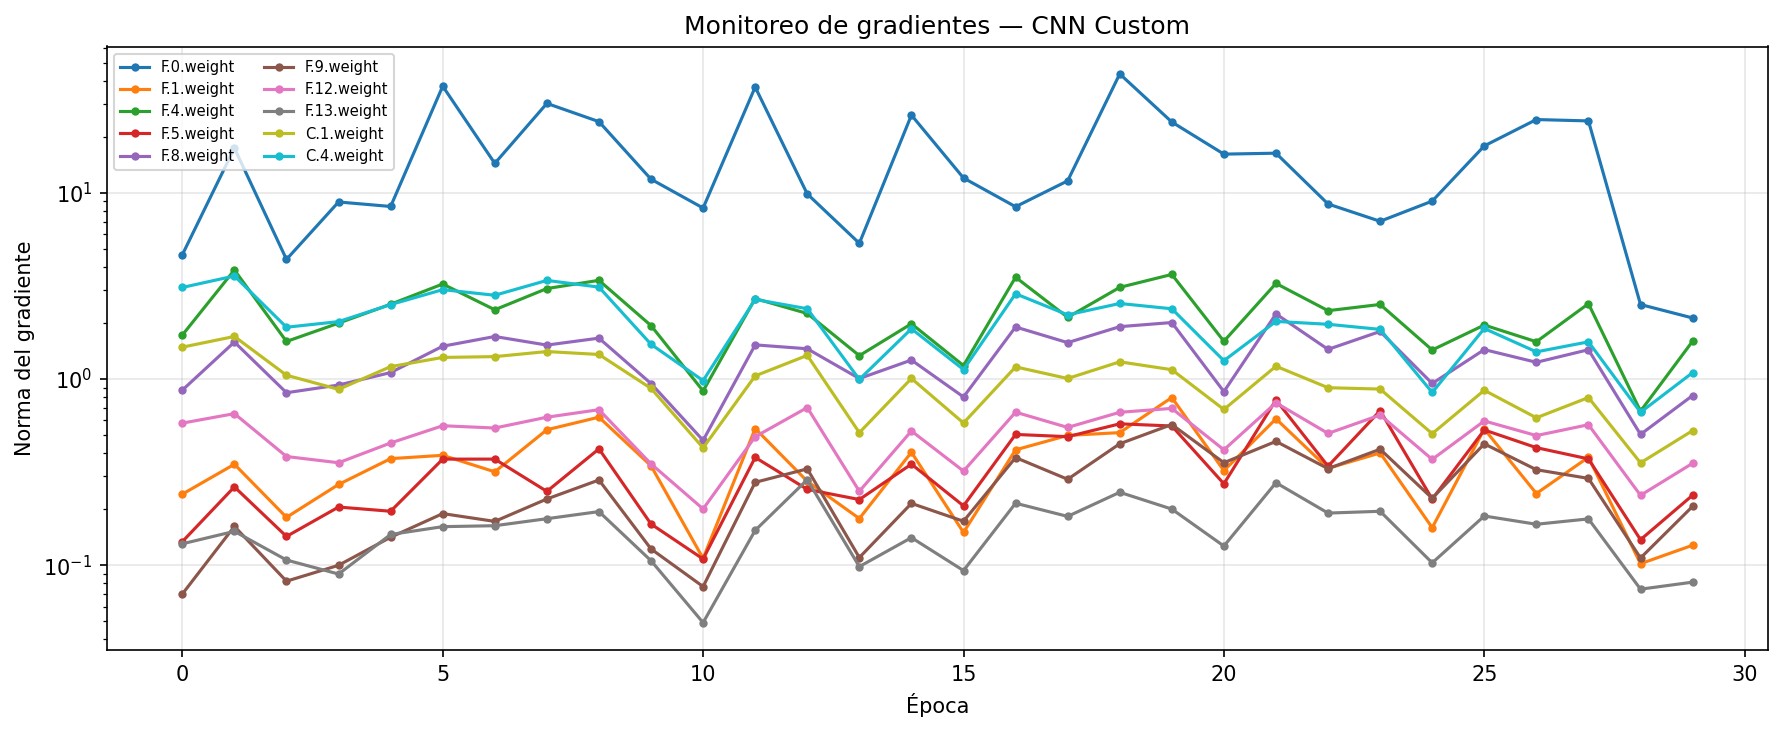
\includegraphics[width=0.68\linewidth]{gradients_cnn_custom.png}
    \caption{Norma del gradiente por capa (escala log). No se observa desvanecimiento ni explosi\'on.}
    \label{fig:grads}
\end{figure}

\section{An\'alisis de errores y espacio latente}

Sobre el conjunto de \textbf{test} la CNN propia alcanza un \textbf{accuracy del 95{,}6\%}
($2581/2700$). La matriz de confusi\'on (Figura~\ref{fig:cm-custom}) muestra que el grueso del error
se concentra entre clases agr\'icolas/vegetaci\'on, visualmente muy parecidas desde un sat\'elite:
\emph{PermanentCrop}$\to$\emph{HerbaceousVegetation} (17 casos), el sentido inverso (9) y
\emph{River}$\to$\emph{AnnualCrop}/\emph{Highway} (cuerpos de agua angostos confundidos con caminos o
parcelas). Clases con textura distintiva (\emph{Forest}, \emph{Residential}, \emph{SeaLake}) son casi
perfectas. Estas confusiones reflejan la ambig\"uedad inherente del uso de suelo, donde las fronteras
entre categor\'ias son difusas.

\begin{figure}[H]
    \centering
    \begin{subfigure}{0.49\textwidth}
        \centering
        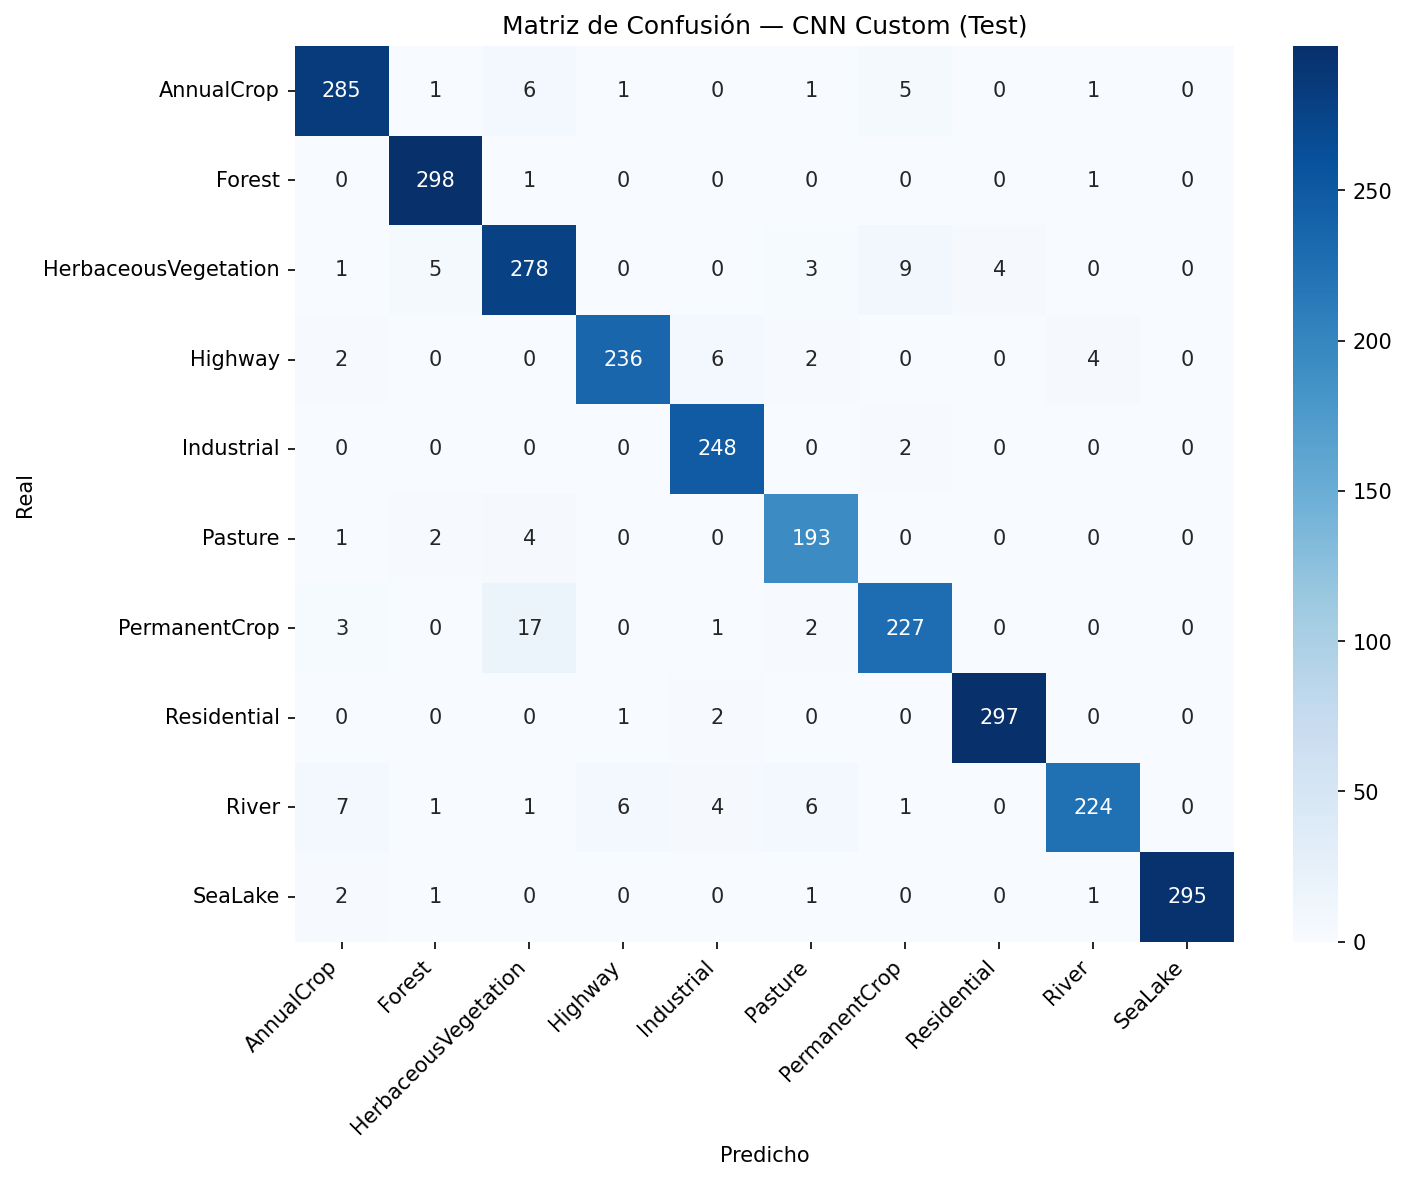
\includegraphics[width=\linewidth]{confusion_matrix_custom.png}
        \caption{Matriz de confusi\'on (test).}
        \label{fig:cm-custom}
    \end{subfigure}\hfill
    \begin{subfigure}{0.49\textwidth}
        \centering
        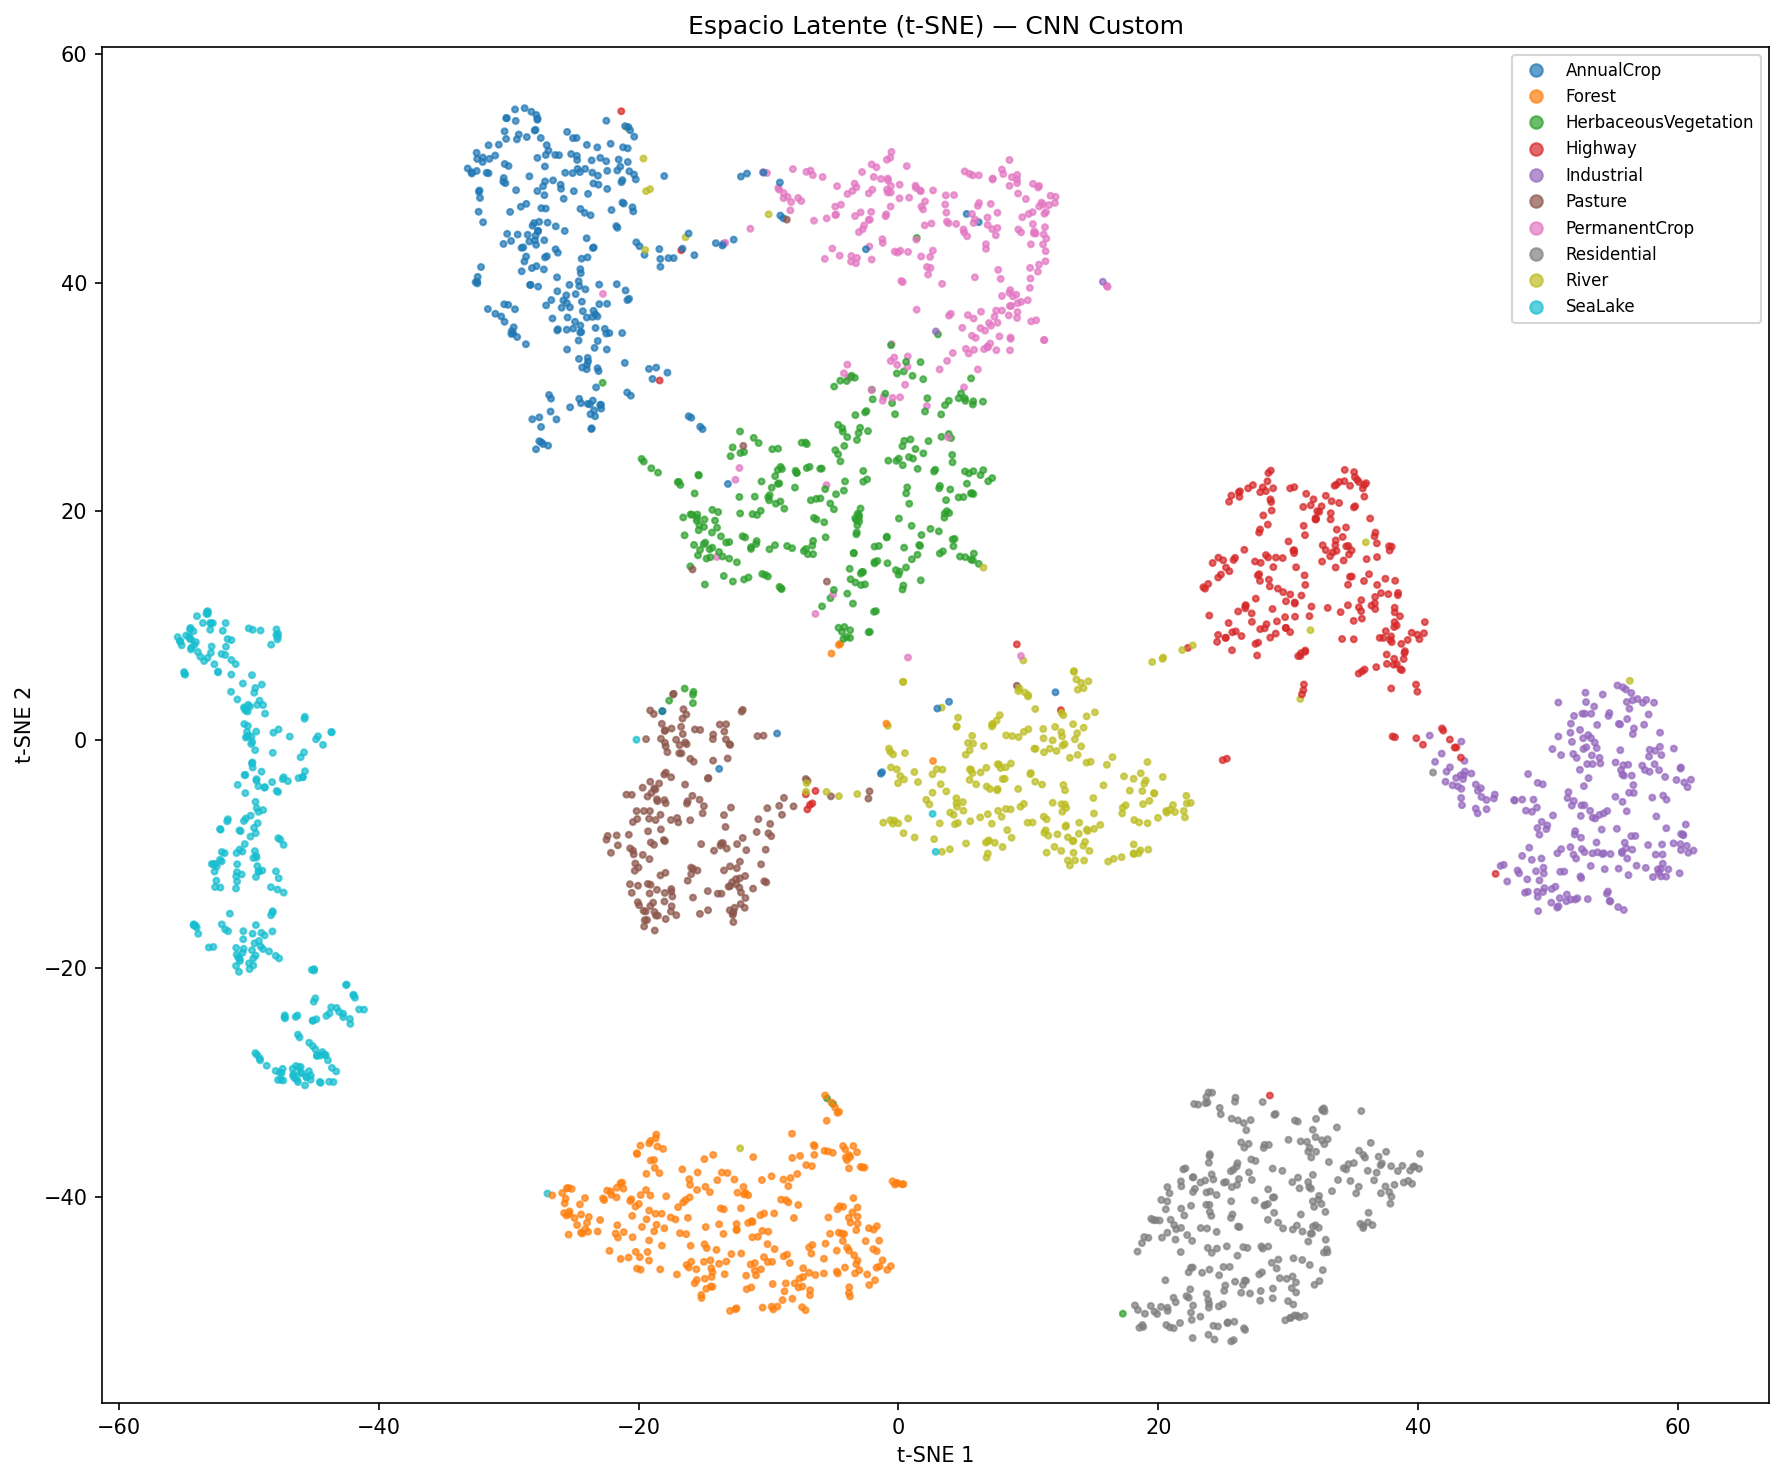
\includegraphics[width=\linewidth]{tsne_custom.png}
        \caption{Espacio latente proyectado con t-SNE.}
        \label{fig:tsne}
    \end{subfigure}
    \caption{An\'alisis de la CNN propia: errores por clase y estructura del espacio latente.}
\end{figure}

\textbf{Espacio latente.} Extrajimos los \emph{features} de 128 dimensiones previos a la capa de
clasificaci\'on y los proyectamos a 2D con t-SNE (Figura~\ref{fig:tsne}). La mayor\'ia de las clases
forman \emph{clusters} distinguibles \emph{antes} de la decisi\'on final, lo que indica que la red
aprendi\'o representaciones discriminativas. Los \emph{clusters} que se solapan
(cultivos/vegetaci\'on) coinciden con las confusiones de la matriz, confirmando que el error proviene
de clases genuinamente similares y no de un fallo de aprendizaje.

\section{Transfer Learning con ResNet18}

Partimos de una \textbf{ResNet18} preentrenada en ImageNet. Aplicamos \emph{fine-tuning} selectivo:
congelamos las capas iniciales y descongelamos solo \texttt{layer4} y reemplazamos la capa final
(\texttt{fc}) por una nueva de 10 salidas con \texttt{Dropout} ($\sim$8{,}4M par\'ametros entrenables de
$\sim$11{,}2M totales). Como ResNet espera entradas de $224\times224$, redimensionamos las im\'agenes.
Entrenamos 15 \'epocas con Adam (\texttt{lr}$=10^{-4}$).

\begin{table}[H]
\centering
\small
\begin{tabular}{lcc}
\toprule
\textbf{M\'etrica} & \textbf{CNN propia} & \textbf{ResNet18 (TL)} \\
\midrule
Accuracy en test            & 95{,}6\%      & \textbf{98{,}0\%} \\
Mejor accuracy en validaci\'on & $\sim$0{,}94 & \textbf{$\sim$0{,}977} \\
\'Epocas para converger     & 30 (ruidosa)  & \textbf{$\sim$3 (estable)} \\
Par\'ametros totales        & 0{,}42 M      & 11{,}2 M \\
Par\'ametros entrenables    & 0{,}42 M      & $\sim$8{,}4 M \\
Costo de c\'omputo / \'epoca & bajo ($64^2$) & alto ($224^2$, $\sim$6$\times$) \\
\bottomrule
\end{tabular}
\caption{Comparaci\'on entre la CNN propia y el \emph{transfer learning} con ResNet18.}
\label{tab:comp}
\end{table}

La Figura~\ref{fig:comp} compara la convergencia de ambos modelos. ResNet18 \textbf{parte ya en
$\sim$0{,}95} de \emph{accuracy} en la primera \'epoca y se estabiliza casi de inmediato, mientras que
la CNN propia necesita decenas de \'epocas ruidosas para acercarse. Esto se debe a que las features de
bajo nivel aprendidas en ImageNet (bordes, texturas, formas) son transferibles al dominio satelital.

\begin{figure}[H]
    \centering
    \begin{subfigure}{0.49\textwidth}
        \centering
        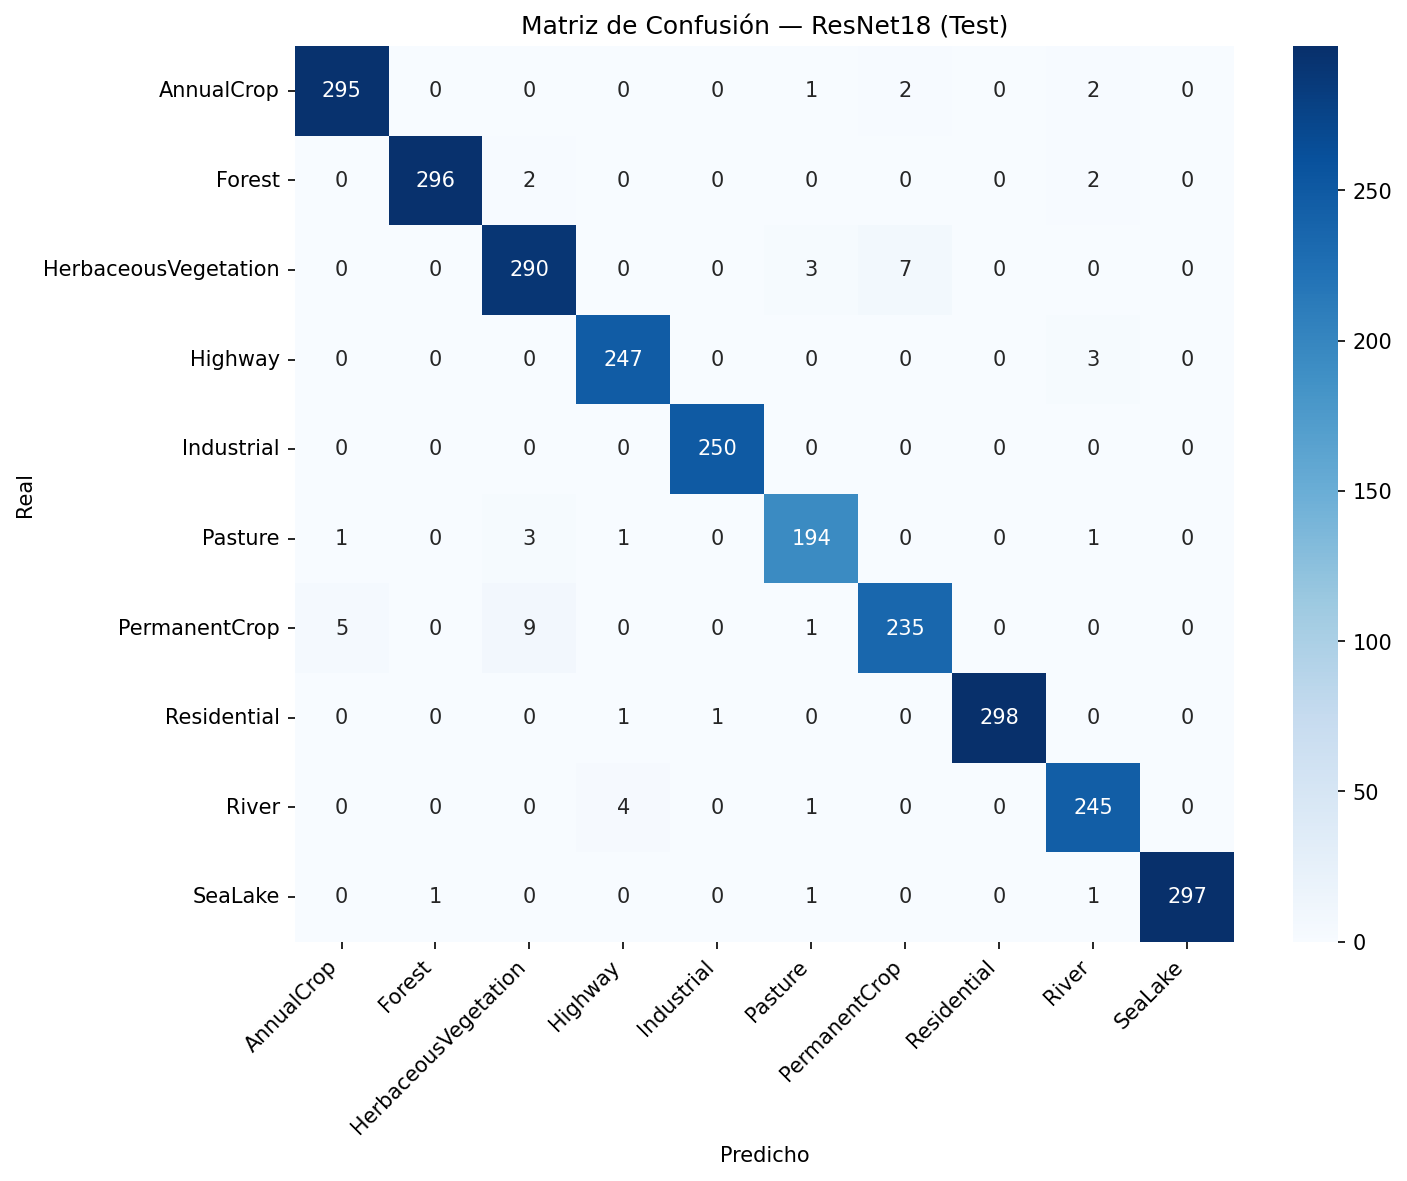
\includegraphics[width=\linewidth]{confusion_matrix_resnet18.png}
        \caption{Matriz de confusi\'on de ResNet18 (test).}
        \label{fig:cm-resnet}
    \end{subfigure}\hfill
    \begin{subfigure}{0.49\textwidth}
        \centering
        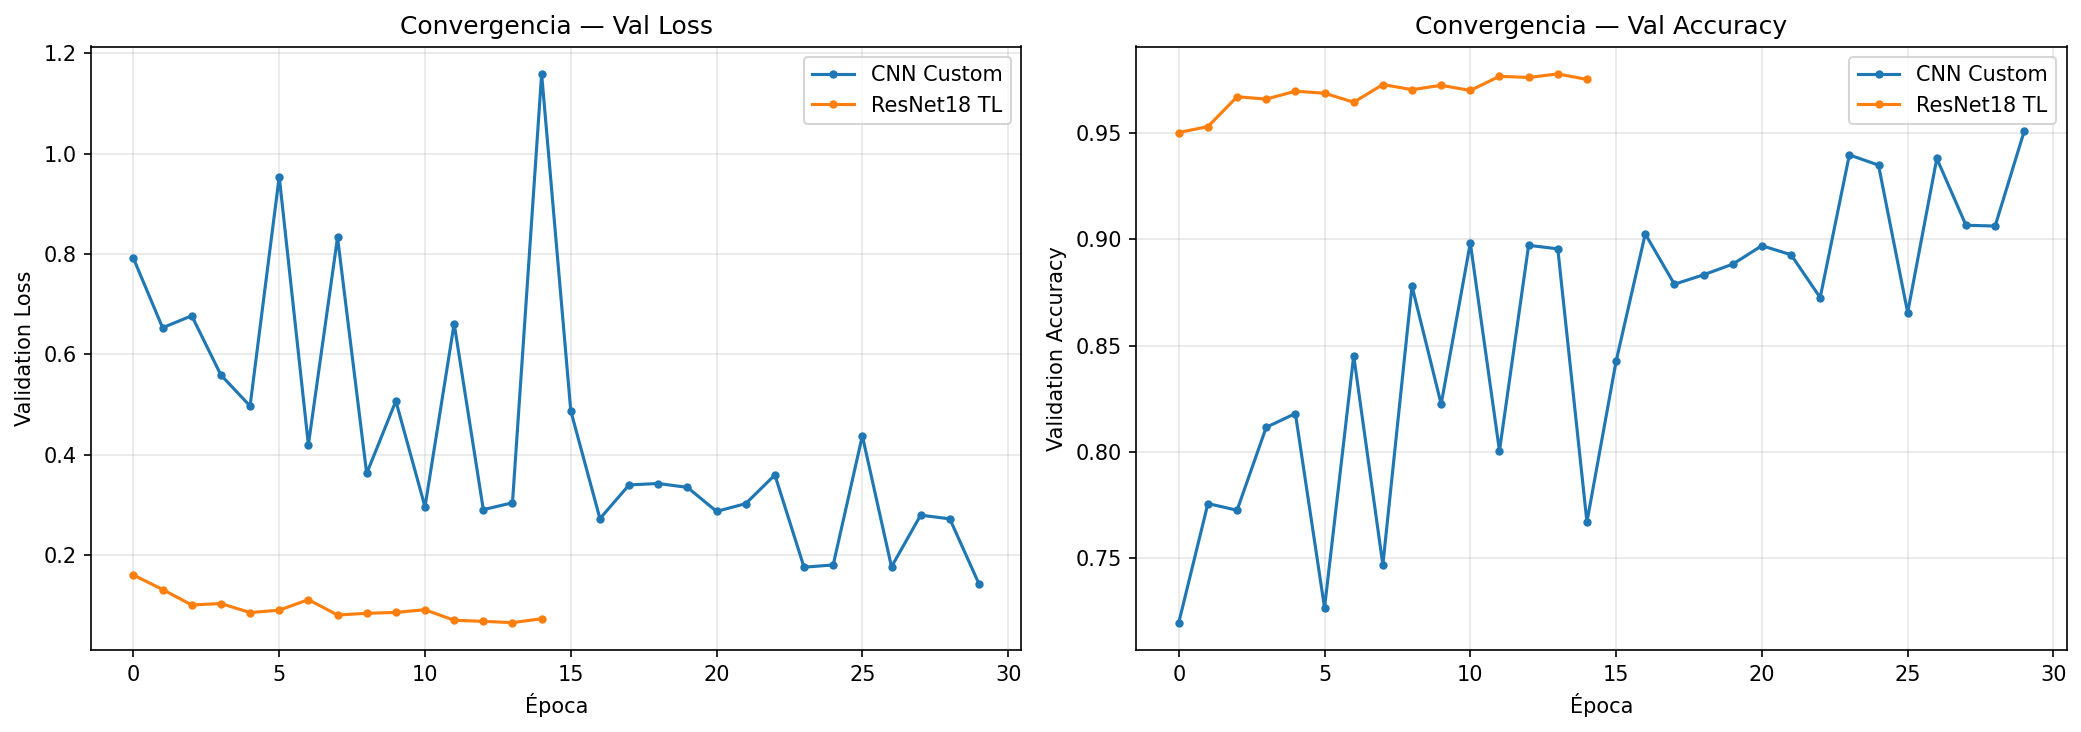
\includegraphics[width=\linewidth]{comparacion_convergencia.png}
        \caption{Convergencia comparada (\emph{val loss} y \emph{val acc}).}
        \label{fig:conv}
    \end{subfigure}
    \caption{Resultados de ResNet18 y comparaci\'on de convergencia con la CNN propia.}
    \label{fig:comp}
\end{figure}

ResNet18 no solo mejora el \emph{accuracy} global sino que \textbf{reduce a la mitad} las confusiones
m\'as dif\'iciles (p.\,ej.\ \emph{PermanentCrop}$\to$\emph{HerbaceousVegetation} baja de 17 a 9 casos),
aunque el solapamiento cultivos/vegetaci\'on persiste por ser intr\'insecamente ambiguo.

\section{Conclusiones}

\begin{itemize}
    \item La CNN propia, con apenas 0{,}42M de par\'ametros, logra un s\'olido 95{,}6\% de
    \emph{accuracy} y un espacio latente bien estructurado, validando el dise\~no.
    \item El \emph{transfer learning} con ResNet18 es superior en todos los ejes salvo el costo por
    \'epoca: converge en pocas \'epocas y alcanza 98{,}0\%, gracias a las features preentrenadas.
    \item El mayor costo por \'epoca de ResNet18 (entradas $224\times224$ y m\'as par\'ametros) se
    compensa con la dr\'astica reducci\'on en la cantidad de \'epocas necesarias.
    \item El \emph{fine-tuning} de solo \texttt{layer4}\,+\,\texttt{fc} es efectivo: conserva las
    features generales de bajo nivel y adapta las de alto nivel al dominio satelital.
\end{itemize}

\end{document}
